%Version 2.1 April 2023
% See section 11 of the User Manual for version history
%
%%%%%%%%%%%%%%%%%%%%%%%%%%%%%%%%%%%%%%%%%%%%%%%%%%%%%%%%%%%%%%%%%%%%%%
%%                                                                 %%
%% Please do not use \input{...} to include other tex files.       %%
%% Submit your LaTeX manuscript as one .tex document.              %%
%%                                                                 %%
%% All additional figures and files should be attached             %%
%% separately and not embedded in the \TeX\ document itself.       %%
%%                                                                 %%
%%%%%%%%%%%%%%%%%%%%%%%%%%%%%%%%%%%%%%%%%%%%%%%%%%%%%%%%%%%%%%%%%%%%%

%%\documentclass[referee,sn-basic]{sn-jnl}% referee option is meant for double line spacing

%%=======================================================%%
%% to print line numbers in the margin use lineno option %%
%%=======================================================%%

%%\documentclass[lineno,sn-basic]{sn-jnl}% Basic Springer Nature Reference Style/Chemistry Reference Style

%%======================================================%%
%% to compile with pdflatex/xelatex use pdflatex option %%
%%======================================================%%

%%\documentclass[pdflatex,sn-basic]{sn-jnl}% Basic Springer Nature Reference Style/Chemistry Reference Style


%%Note: the following reference styles support Namedate and Numbered referencing. By default the style follows the most common style. To switch between the options you can add or remove “Numbered” in the optional parenthesis. 
%%The option is available for: sn-basic.bst, sn-vancouver.bst, sn-chicago.bst, sn-mathphys.bst. %  
 
%%\documentclass[sn-nature]{sn-jnl}% Style for submissions to Nature Portfolio journals
%%\documentclass[sn-basic]{sn-jnl}% Basic Springer Nature Reference Style/Chemistry Reference Style
\documentclass[sn-mathphys,Numbered]{sn-jnl}% Math and Physical Sciences Reference Style
%%\documentclass[sn-aps]{sn-jnl}% American Physical Society (APS) Reference Style
%%\documentclass[sn-vancouver,Numbered]{sn-jnl}% Vancouver Reference Style
%%\documentclass[sn-apa]{sn-jnl}% APA Reference Style 
%%\documentclass[sn-chicago]{sn-jnl}% Chicago-based Humanities Reference Style
%%\documentclass[default]{sn-jnl}% Default
%%\documentclass[default,iicol]{sn-jnl}% Default with double column layout

%%%% Standard Packages
%%<additional latex packages if required can be included here>

\usepackage{graphicx}
\usepackage{multirow}
\usepackage{amsmath,amssymb,amsfonts}
\usepackage{amsthm}
\usepackage{mathrsfs}
\usepackage[title]{appendix}
\usepackage{xcolor}
\usepackage{textcomp}
\usepackage{manyfoot}
\usepackage{booktabs}
\usepackage{algorithm}
\usepackage{algorithmicx}
\usepackage{algpseudocode}
\usepackage{listings}
\usepackage{soul}   % For the \hl{} command, which highlights text. William uses this to remind himself that something needs to be revised.
\usepackage{outlines}   % For multi-level lists

% For flow diagram
\usepackage{tikz}
\usetikzlibrary{shapes, arrows, positioning}
\tikzstyle{compartment} = [circle, minimum width=1cm, text centered, draw=black, fill=none]
\tikzstyle{hidden} = [circle, minimum width=0.5cm, text centered, draw=none, fill=none]
\tikzstyle{arrow} = [thick,->,>=stealth]

% Shorthand for compartment names. Prefix ``c'' denotes ``compartment''
\newcommand{\cX}{\mathbf{X}}
\newcommand{\cE}{\mathbf{E}}
\newcommand{\cL}{\mathbf{L}}
\newcommand{\cT}{\mathbf{T}}
\newcommand{\cR}{\mathbf{R}}


%%%%%=============================================================================%%%%
%%%%  Remarks: This template is provided to aid authors with the preparation
%%%%  of original research articles intended for submission to journals published 
%%%%  by Springer Nature. The guidance has been prepared in partnership with 
%%%%  production teams to conform to Springer Nature technical requirements. 
%%%%  Editorial and presentation requirements differ among journal portfolios and 
%%%%  research disciplines. You may find sections in this template are irrelevant 
%%%%  to your work and are empowered to omit any such section if allowed by the 
%%%%  journal you intend to submit to. The submission guidelines and policies 
%%%%  of the journal take precedence. A detailed User Manual is available in the 
%%%%  template package for technical guidance.
%%%%%=============================================================================%%%%


%% as per the requirement new theorem styles can be included as shown below
\theoremstyle{thmstyleone}%
\newtheorem{theorem}{Theorem}%  meant for continuous numbers
%%\newtheorem{theorem}{Theorem}[section]% meant for sectionwise numbers
%% optional argument [theorem] produces theorem numbering sequence instead of independent numbers for Proposition
\newtheorem{proposition}[theorem]{Proposition}% 
%%\newtheorem{proposition}{Proposition}% to get separate numbers for theorem and proposition etc.

\theoremstyle{thmstyletwo}%
\newtheorem{example}{Example}%
\newtheorem{remark}{Remark}%

\theoremstyle{thmstylethree}%
\newtheorem{definition}{Definition}%

\raggedbottom
%%\unnumbered% uncomment this for unnumbered level heads

 \graphicspath{ {./sensitivity xx3/} }
\begin{document}

\title[Article Title]{Dynamical Models of Tuberculosis among Canadian Immigrants}

%%=============================================================%%
%% Prefix	-> \pfx{Dr}
%% GivenName	-> \fnm{Joergen W.}
%% Particle	-> \spfx{van der} -> surname prefix
%% FamilyName	-> \sur{Ploeg}
%% Suffix	-> \sfx{IV}
%% NatureName	-> \tanm{Poet Laureate} -> Title after name
%% Degrees	-> \dgr{MSc, PhD}
%% \author*[1,2]{\pfx{Dr} \fnm{Joergen W.} \spfx{van der} \sur{Ploeg} \sfx{IV} \tanm{Poet Laureate} 
%%                 \dgr{MSc, PhD}}\email{iauthor@gmail.com}
%%=============================================================%%

\author*[1]{\fnm{Jeremy} \sur{Chiu}}\email{jeremychiu@langara.ca}

\author[2]{\fnm{William} \sur{Ruth}}\email{william\_ruth@sfu.ca}
\equalcont{These authors contributed equally to this work.}

\author[1]{\fnm{Albert} \sur{Wong}}\email{alwong@langara.ca}
\equalcont{These authors contributed equally to this work.}

\author[1]{\fnm{Timothy} \sur{Lee}}\email{tlee74@mylangara.ca}

\author[1]{\fnm{Kezia} \sur{Wijaya}}\email{kwijaya01@mylangara.ca}

\affil*[1]{\orgdiv{Mathematics and Statistics}, \orgname{Langara College}, \orgaddress{\street{100 E. West 49th Avenue}, \city{Vancouver}, \postcode{V5Y 2Z6}, \state{B.C.}, \country{Canada}}}

\affil[2]{\orgdiv{Statistics}, \orgname{Universite de Montreal}, \orgaddress{\street{2900, boul. Édouard-Montpetit}, \city{Montreal}, \postcode{H3T 1J4}, \state{PQ}, \country{Canada}}}


%%==================================%%
%% sample for unstructured abstract %%
%%==================================%%

\abstract{This research developed a dynamical system model for the Canadian immigrants for the ten year period between 2011 and 2020.}

%%================================%%
%% Sample for structured abstract %%
%%================================%%

% \abstract{\textbf{Purpose:} The abstract serves both as a general introduction to the topic and as a brief, non-technical summary of the main results and their implications. The abstract must not include subheadings (unless expressly permitted in the journal's Instructions to Authors), equations or citations. As a guide the abstract should not exceed 200 words. Most journals do not set a hard limit however authors are advised to check the author instructions for the journal they are submitting to.
% 
% \textbf{Methods:} The abstract serves both as a general introduction to the topic and as a brief, non-technical summary of the main results and their implications. The abstract must not include subheadings (unless expressly permitted in the journal's Instructions to Authors), equations or citations. As a guide the abstract should not exceed 200 words. Most journals do not set a hard limit however authors are advised to check the author instructions for the journal they are submitting to.
% 
% \textbf{Results:} The abstract serves both as a general introduction to the topic and as a brief, non-technical summary of the main results and their implications. The abstract must not include subheadings (unless expressly permitted in the journal's Instructions to Authors), equations or citations. As a guide the abstract should not exceed 200 words. Most journals do not set a hard limit however authors are advised to check the author instructions for the journal they are submitting to.
% 
% \textbf{Conclusion:} The abstract serves both as a general introduction to the topic and as a brief, non-technical summary of the main results and their implications. The abstract must not include subheadings (unless expressly permitted in the journal's Instructions to Authors), equations or citations. As a guide the abstract should not exceed 200 words. Most journals do not set a hard limit however authors are advised to check the author instructions for the journal they are submitting to.}

\keywords{Tuberculosis, Dynamical Models, Canadian Immigrants}

%%\pacs[JEL Classification]{D8, H51}

%%\pacs[MSC Classification]{35A01, 65L10, 65L12, 65L20, 65L70}

\maketitle

\section{Introduction}\label{sec1}

We will write this section last

\begin{outline}
    \1 Literature review -- biology of TB, Canadian foreign-born population and screening and immigration (with TB), mathematics 
    \1 Model. Theirs (Guo \& Wu) without any adaptations
        \2 Data
    \1 Show problems with their model: 
        \2 calculate incidence, it's very off [Fig2, top graph]
        \2 $R_0=0$ has problems.
    \1 Optimization using fmincon, their parameters
        \2 $R_0$ same problem
        \2 we include $L_0$ as an optimization (estimated) parameter, but it's extremely dependent on our ``initial choice" of $L_0$.  The optimized $L_0$ stays nearly identical to our initial choice
    \1 Other graphs:
        \2 Sensitivity analysis for $\nu$ and $\omega$ (and many other parameters that don't really matter)
        \2 After sensitivity analysis, we inspect the combinations of parameters that yield low error
        \2 plot error vs (certain) parameter
        \2 post-sensitivity analysis, we have distributions of optimal $q_1,~q_2,~E_0,~ L_0,~ R_0$
        \2 how to pick $L_0$
        \2 (?) updating $L_0$ at every step causes problems in that optimizer no longer changes $E_0$
    \1 other model updates:
        \2 arrows pointing from $R$ to $T$
\end{outline}

\section{Literature Review}\label{sec2}

Background and TB in general

WHO report on TB (number of cases) \cite{WHO2022Global2022}

Canadian numbers and recent studies

Canada TB numbers \cite{MounchiliA.2022TuberculosisReport} and \cite{Long2020TuberculosisCanada}

Canadian context \cite{Ronald2018DemographicStudy} and \cite{CollegeofFamilyPhysiciansofCanada.2017TuberculosisCanada} and \cite{Essue2018BetterCanada}

Canadian communities \cite{Tuite2017StochasticCommunities} and \cite{Amiri2021SpatialCanada} \cite{Zwick2021RepresentingApproach}

Canadian Immigrant population \cite{Ng2018HealthCanada}

TB Modelling
SIIR Model for South Sulawesi \cite{Side2023TheSulawesi}
VSEIT Model for Algeria \cite{Chennaf2023AnalysisEffects}
SIS-SEIS Model for Indonesia \cite{Maulana2022ParameterIndonesia}
SEII model \cite{Permatasari2022MATHEMATICALINFECTION}
SELT Model with early and late latency \cite{Guo2006GlobalTuberculosis}

Impact of immigrants \cite{Inigo2007AnalysisImmigration}

Reinfection
Contribution of reinfection to ARI and incidence of TB \cite{Horsburgh2022ContributionDisease}
SEIRE Model\cite{Sulayman2023DynamicsIssues}


\subsection{Papers and work that heavily influence our work}

Guo paper on the basic model with early and late latency and  without re-infection \cite{Guo2011PersistentLatency}

TB Surveillance reports, which include data we use \cite{MounchiliA.2022TuberculosisReport}

\subsection{In 2008 to 2020, what countries did Canadian immigrants come from}

See Wikipedia.

This shows that a significant proportion of Canada’s recent immigrants are from TB high-incidence countries, e.g. India \cite{Varshney2023TrendsPandemic}, China \cite{Yu2020Estimating2025-2050}, and Philippines\cite{Capeding2022Cost2017}.

\subsection{[TIM] Screening Procedure in Canada (and other low-incidence countries} 
       
       %ACTIVE TB DISEASE DETECTION 
     In Canada, the primary detection method for active Tuberculosis disease is a series of diagnostic tests consisting of a chest radiography, followed by an MRI or similar scans, as well as a test for microbiological TB presence via sputum samples (Public Health Agency of Canada [PHAC],2014). The chest radiography involves scanning the lungs for abnormalities that have been observed in high proportions of previous confirmed cases of tuberculosis disease (Canadian Thoracic Society [CTS], 2019). For example, 56.2 percent of previously confirmed positive TB cases were observed to have varying degrees of cavitation in the upper lungs (CTS, 2019). Other abnormalities include, but are not limited to, calcified pulmonary modules, intrathoracic adenopathy, and fluid accumulation in the pleural cavity (CTS, 2019). These abnormalities are statistically \textit{associated} with active pulmonary TB, but are not exclusively TB symptoms. (CTS, 2019). To err on the side of caution, all documented abnormalities should be looked for during screening, as to minimize false negative diagnoses. As a result, the chest radiography has a fairly high sensitivity estimated to be over 0.95 when considering all associated lung irregularities, but has a specificity as low as 0.75 (CTS, 2019). % please see explanation for specificity/sensitivity in TIM Literature folder. I believe they are pretty commonly used measures of diagnostic test accuracy in epidemiology.
     To improve specificity, individuals tested positive for the chest radiograph are required to undergo sputum testing to confirm the diagnosis (PHAC, 2014). MRI and other scans are also performed in conjunction to detect for extra-pulmonary tuberculosis and further increase specificity (CTS, 2019).  Extra-pulmonary TB is assumed to have no mechanism for for transmission, and so is not transmissible from an infected host \cite{InfectiousHandbook}.

    %LATENT TB Infection (LBTI) DETECTION
          The tuberculin skin test (TST) and interferon gamma release assay (IGRA) are used to detect latent TB infection, but yield a positive result for both LTBI and active TB (CTS, 2019). TST is an \textit{in vivo} examination in which tuberculin, proteins which contain \textit{M. Tuberculosis} antigen, is injected into the skin of the testing patient. The localized region of skin is observed for reactions after 48-72 hours, which is indicative of prior infection (PHAC, 2014). The degree of swelling of the skin region is examined, with a >5mm rise in the skin being considered the threshold for a positive latent TB diagnosis, while any changes under 5mm is generally considered negative (CTS, 2019). 
    On the other hand, IGRA test is an \textit{in vitro} test which involves injecting blood samples with \textit{M. Tuberculosis} antigen (PHAC, 2014). Immune responses from adapted T cells will emit a protein known as Interferon-gamma (Tau \& Rothman, 1999), which is a litmus for infection if detected in the blood sample above a certain threshold (>0.35IU/mL) (CTS, 2019). It should be noted that the thresholds for both tests were chosen to balance specificity and sensitivity, but can be raised or lowered to maximize one over the other (CTS, 2019). For example, if a rise of skin over 10 mm were considered a positive diagnosis in the skin test rather than 5mm, then there would be less false positive diagnoses, but more false negatives as a result (increasing specificity for a decrease in sensitivity) (CTS, 2019). The thresholds used in TST and IGRA are loosely standardized, and may vary by medical practitioner (CTS, 2019). Furthermore, immunizations have been shown to cause false negatives (PHAC, 2014), and other diseases (including active TB disease) can cause false positives in LBTI tests (CTS, 2019). As a result, both TST and IGRA tests have relatively low sensitivity as well as specificity (CTS, 2019).

          %Screening and Immigration Policy
     According to \textit{Canadian Tuberculosis Standards 7th Edition: 2014}, all permanent migrants %I believe pre-entry "permanent residents" are individuals who were approved for a permanent Canadian visa pre-immigration, in which case the PR card would be provided shortly after landing. People on temporary work Visas, school, or on extended stays can apply for PR later on, but they are considered temporary residents or visitors when travelling to Canada. If their stays are longer than 6 months they will undergo similarl to screening permenent migrants, will discuss ->
     are required to be undergo chest radiography to be scdreened for active tuberculosis disease. Any positive tests must undergo further diagnosis and necessary treatment before allowed entry (PHAC, 2014). For visitors /temporary migrants, individuals who are on extended stays of over 6 months, come from high incidence countries with over 30/100000 TB incidence rates, or have healthcare-related occupations are also screened for active TB pre-entry (PHAC, 2014). LBTI screening is not performed en masse for migrant groups pre-entry, and is instead performed on \textit{select} migrants who are at higher risk to have been exposed to TB infection (PHAC, 2014). The incidence rate in the country of origin, proximity to active cases, and occupation are factors used to assess risk and selection for LBTI screening (PHAC, 2014). Those who are tested positive for LBTI are still allowed entry, but are subject to medical surveillance (PHAC, 2014). As of the 8th edition of the Canadian Tuberculosis Standards, LBTI tests are still discouraged for mass screening migrants due to its cost:benefit ratio, and reserved for high risk travellers (CTS, 2019).

    
     % some data I ran across that might be useful and implications
     -On average, Canada receives ~280 000 permanent resident arrivals and ~380 000 temporary resident arrivals per year, with 70 percent of entries being from high incidence countries (PHAC, 2014). In 2011, of the 500992 pre-entry medical tests, 0.09 percent resulted in positive for active TB disease (PHAC, 2014)
     
     -only ~69 percent of arrivals were tested for LBTI before \textit{or} after entry. This lack of mass screening for LBTI, as well as the lack of accuracy in the LBTI tests described earlier, are likely the main reasons why data regarding migrants w/ LBTI is not well-documented, and is the main crux of this paper. %that being said, as per the 2014 Canadian TB Standards, 53-61 percent of tuberculin skin tests on adults from high risk countries were positive for LBTI (PHAC, 2014). This however, does not reflect the whole migrant population, since the people required to take LBTI tests are the ones who were considered to have a high probability of infection -> selection bias

     

 

\subsection{TB Reactivation - relapse and reinfection [Kezia, add to this]}

Patients who develop active Tuberculosis more than once in their lifetime can be classified into one of two categories -- exogenous reinfection, or endogenous relapse / reactivation. Cases of relapse are usually linked with drug resistance, commonly found within the first 2 years after treatment ends \cite{Zong2018RelapseChina} \cite{Guerra-Assunção2015RecurrenceFollow-up}. Two Tuberculosis treatment trials conducted in the United States and Canada found that 96\% of recurrent Tuberculosis cases were from reactivation of the initial infecting strain\cite{Benator2002RifapentineTrial}\cite{Vernon1999AcquiredConsortium}, see also \cite{Jasmer2004RecurrentReinfection} . Although some sources claim reinfection is more common than expected \cite{Hoey2002CanTwice}, the proportion of recurrent TB cases due to relapse or reinfection is highly associated with the respective country. Cases of TB reinfection are often linked with the coexistence of HIV \cite{Campbell2022ChapterInfection.}. 

\cite{Brooks-Pollock2011} ``We observed a saturation effect in the number of cases per household and estimated that protective immunity conferred up to 35\% reduction in the risk of disease."

\cite{Mulberry2020} ``the protection afforded to hosts against a new infection from an established one, ... in a population are hard to estimate and cannot be observed directly."  


\section{The Compartmental Model}\label{sec3}

\citet{Guo2011PersistentLatency} present a sophisticated compartmental model for the spread of tuberculosis (TB) within the foreign-born population\footnotemark of Canada. We adopt the structure of their model, but update their parameter values based on more current data. In this section, we first present the model of \citeauthor{Guo2011PersistentLatency}, then give our updated parameter values. We were unable to locate reasonable values for some parameters. We discuss our approach to these unknown parameters in Section \ref{sec:data_pars}.

\footnotetext{Depending on the source, there may or may not be a difference between the terms ``foreign-born'' and ``immigrant''. In practice, the operational definition must be checked for each source, regardless of which term is used. In this work, we use the terms interchangeably, and define them both to mean ``something'' (\hl{we need to be careful and precise about this definition. We may actually not be able to get away with a single definition, in which case we can mention the inconsistency of what is being measured as a limitation of our study in the Discussion section}).}

The model used by \citeauthor{Guo2011PersistentLatency} to model TB transmission divides people into five compartments based on their disease status: Susceptible ($\cX$), Early Latent ($\cE$), Late Latent ($\cL$), Active ($\cT$) and Recovered ($\cR$). In brief, individuals begin their life susceptible. A person may become infected upon contact with an active TB case. Immediately after infection, an individual moves to the early latent stage \hl{(the \textit{latent period} is defined as time from infection to infectiousness\cite{InfectiousHandbook})}. From here, they may progress either to late latent or to active TB. After entering the late latent stage, individuals move to active infection after some time. Finally, active cases progress to recovered. 



Discuss $E$ vs $L$.  $E$ means 2 years, not ``before TB becomes dormant." Cite standards 7th edition.

Our model also incorporates demography. That is, individuals can be born (enter the system) and die (leave the system). In our case, birth corresponds to immigration, while death is interpreted literally. We assume that an immigrant may be susceptible or latent, but that the immigration screening process excludes all active cases. We also allow for individuals in any compartment to die, and assume each compartment's death rate is the same (aside for the Active $T$ compartment, which has an additional death-rate to model death due to TB).

\subsection{Equations}

[awk] All the assumptions give rise to the following system of differential equations.

\begin{equation}
    \begin{cases}
        X' &= (1-q_1-q_2)\pi - \beta X \cT - d_X X, \\
        E' &= q_1 \pi + \beta XT - (d_e+\omega)E,\\
        L' &= q_2 \pi + (1-p)\omega E - (d_L + \nu) L,\\
        T' &= pwE + \nu L -(d_T+\alpha+\delta) T \\
        R' &= dT - d_R R
    \end{cases}
    \label{eq:model}
\end{equation}

Figure \ref{fig:flow} gives a diagram of our compartments, along with arrows and rates for all possible transitions. Table \ref{tab:pars} gives more detail on each of the parameters in our model, and Table \ref{tab:init} gives the initial conditions used for our model. Note that some parameters and initial conditions are pulled from the literature, while others are estimated from the data.

\begin{figure}[tpb]
    \centering
    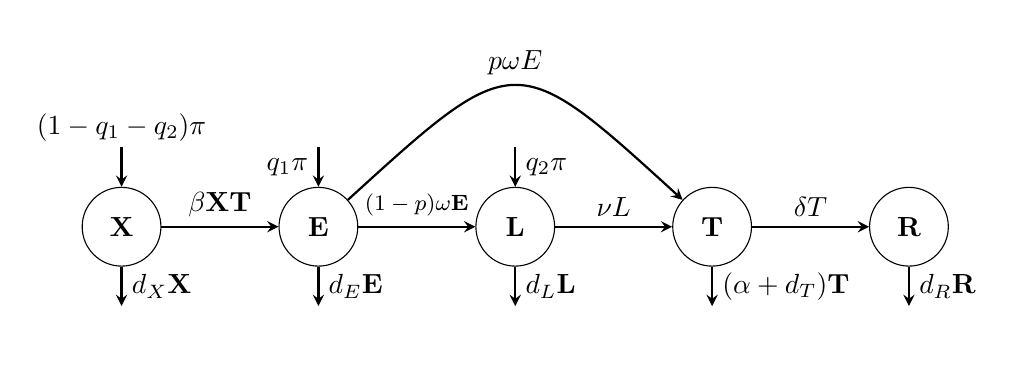
\begin{tikzpicture}[node distance = 2.5cm]
        \node (X) [compartment] {$\cX$};
        \node (E) [compartment, right of=X] {$\cE$};
        \node (L) [compartment, right of=E] {$\cL$};
        \node (T) [compartment, right of=L] {$\cT$};
        \node (R) [compartment, right of=T] {$\cR$};
        \draw [arrow] (X) --  node[align=center, above] {$\beta \cX \cT$} (E);
        \draw [arrow] (E) -- node[align=center, above] {\color{black} \footnotesize $(1 - p) \omega \cE$} (L); % May need to adjust size for final version
        \draw [arrow] (L) -- node[align=center, above] {$\nu L$} (T);
        \draw [arrow] (T) -- node[align=center, above] {$\delta T$} (R);
        % Invisible nodes above and below each compartment for birth/death rates
        \node (aX) [hidden, above=0.5cm of X] {};
        \node (aE) [hidden, above=0.5cm of E] {};
        \node (aL) [hidden, above=0.5cm of L] {};
        \node (bX) [hidden, below=0.5cm of X] {};
        \node (bE) [hidden, below=0.5cm of E] {};
        \node (bL) [hidden, below=0.5cm of L] {};
        \node (bT) [hidden, below=0.5cm of T] {};
        \node (bR) [hidden, below=0.5cm of R] {};
        % Arrows representing birth and death
        \draw [arrow] (aX) node[align=center] {$(1 - q_1 - q_2) \pi$} --  (X);
        \draw [arrow] (aE) -- node[align=center, left] {$q_1 \pi$} (E);
        \draw [arrow] (aL) -- node[align=center, right] {$q_2 \pi$} (L);
        \draw [arrow] (X) -- node[align=center, right] {$d_X \cX$} (bX);
        \draw [arrow] (E) -- node[align=center, right] {$d_E \cE$} (bE);
        \draw [arrow] (L) -- node[align=center, right] {$d_L \cL$} (bL);
        \draw [arrow] (T) -- node[align=center, right] {$( \alpha+d_T ) \cT$} (bT);
        \draw [arrow] (R) -- node[align=center, right] {$d_R \cR$} (bR);
        % Arrow representing skipping the late latent stage (i.e. from E to T)
        \node (aaL) [hidden, above=0.5cm of aL] {}; % Invisible node for jumping high enough above L
        \draw [arrow] (E) .. node[align=center, above] {$p \omega E$} controls (aaL) .. (T);
        
    \end{tikzpicture}
    \caption{Flow diagram for our model of TB transmission.}
    \label{fig:flow}
\end{figure}

\begin{table}
    \centering
    \begin{tabular}{ccc}
        Parameter & Description & Value \\
        \hline
        $\pi$ & Annual Immigration Rate & reported \cite{https://www150.statcan.gc.ca/n1/pub/11-630-x/11-630-x2016006-eng.htm}\\
        $q_1$ & Proportion of Early Latent Cases Among Immigrants & Estimated \\
        $q_2$ & Proportion of Late Latent Cases Among Immigrants & Estimated \\
        $\beta$ & TB Transmission Rate & \\
        $d_C$ & Death Rate for Compartment $\mathbf{C}$ & \\
        $\omega$ & Rate of Progressing Past Early Latent Stage & \\
        $p$ & Fraction of Cases Which Skip Late Latent Stage &\\
        $v$ & Rate of Progressing Past Late Latent Stage &\\
        $\delta$ & Recovery Rate from Active TB&
    \end{tabular}
    \caption{Parameters of our model, as well as their specified values and corresponding references. Parameters for which we were unable to find suitable references are labelled as ``estimated''.}
    \label{tab:pars}
\end{table}

\begin{table}
    \centering
    \begin{tabular}{ccc}
    Compartment & Description & Value\\
    \hline
    $\cX_0$ & Susceptible & \\
    $\cE_0$ & Early Latent & Estimated\\
    $\cL_0$ & Late Latent & Estimated\\
    $\cT_0$ & Active TB & Reported \\
    $\cR_0$ & Recovered & 
    \end{tabular}
    \caption{Initial conditions for compartment sizes (i.e. size in 2010). Values are either given (with references) or are labelled as ``estimated''.}
    \label{tab:init}
\end{table}

See \citet{Guo2011PersistentLatency} for a detailed stability analysis of this model.


\subsection{Biology and Parameters for Simulation}
\label{sec:data_pars}

\subsubsection{Infectivity $\beta$}

 \cite{Guo2011PersistentLatency} use $\beta=1\times 10^{-8}$, while \cite{Ziv2001EarlyInfection} use $\beta=7\times 10^{-6}$.

\subsubsection{Latent Tuberculosis}

Parameters that relate to the $E$ and $L$ compartment.  $q_1,~q_2,~p,~\omega,~\nu$.  



\cite{Ziv2001EarlyInfection} uses $\nu = 0.00256$, which corresponds to 5 percent probability of development of disease over 20 years during the long-term LTBI stage.  




Many TB infections remain latent and never develop to active TB -- \cite{Khajanchi2018DynamicsReactivation} estimate only 5-10\% of latently infected individuals develop active TB.  

\cite{Brooks-Pollock2011}: ``The mean waiting time between first and second diagnoses in households with ≤7 adults was 3.5 years, and the distribution was skewed toward shorter times, with a median interval between cases of 1.65 years" 

Newly infected patients ($\leq2$ years from infection) are $15\times$ more likely to develop active TB than people with no known risk factor \cite{PublicHealthAgencyofCanada2014CanadianStandards.} (note the 2022 Standards \cite{Campbell2022ChapterInfection} do not report this number ; hence we use the 2014 Standards \cite{PublicHealthAgencyofCanada2014CanadianStandards.} reported number).  Thus $$ p\omega = 15 \cdot \nu  $$

\cite{Jacquet2006} report $p=5\%$, with a range of $2\%-15\%$.

% Immigrant population data - Statistics Canada.
% $$ ReportedTB = [14.6 14.4 14.1 14.7 14.6 15 14.3 15 15.5 15 14.8 15.9 14.3]$$ %Actual TB rate from 2008 - 2020


 $$ ReportedImmigration = [x x 259110 260036 263101 267924 240763 323192 272707 303325 313601 284157 226309] $$

% Incident rate data

%Parameter values for simulations of the compartmental TB model (1) with early and late latently-infected new immigrants.

\section{Analysis}

The parameters of our model are broadly divided into two groups: those obtained from the literature, and those we estimate. Our analysis treats these groups separately. We begin by fixing all unestimated parameters at plausible values. We then optimize over the estimated parameters, calibrating our model to match observed TB incidence. Finally, we investigate sensitivity to our choices of unestimated parameter values by repeating the above process with several different values for each unestimated parameter (\hl{awk}). In this section, we describe our treatment of the unestimated and unestimated parameters in more detail, and discuss what outputs we extract from our individual simulations and sensitivity analysis.

\subsection{Estimation}
\label{sec:estimation}
\hl{Citations needed for methodology. I have some I can use for optimization, but it's worth looking into how Matlab likes to be cited.}

We begin with the estimated parameters, $q_1$, $q_2$, $\cE_0$ and $\cL_0$. For fixed values of the non-estimated parameters, we estimate $q_1$, $q_2$, $\cE_0$ and $\cL_0$ my minimizing the least-squares error for the observed incidence rate of TB among foreign-born individuals in Canada between the years of \hl{2010 and 2020 (confirm this)}. More precisely, for particular values of the non-estimated parameters, we use the \texttt{ode23} function in \texttt{Matlab} \hl{(citation for Matlab? for ode23?)} to solve System \ref{eq:model}. This solution consists of trajectories for the sizes of the compartments in our model. We then compute the TB incidence at each time point using the expression in \citet{Guo2011PersistentLatency}: $pwE +vL$. Our objective function is the squared $\mathcal{L}^2$ difference between predicted and observed incidence at each time point where we have data (\hl{normalization?}). 

Optimization is performed using the \texttt{fmincon} function in \texttt{Matlab}. This function iteratively attempts to take a ``direct step'', in which the KKT equations are approximated using the finite difference method, then linearized and solved. Alternatively, if the Hessian obtained from the finite difference method is not positive definite, the Conjugate Gradient method is used instead for the current iteration.

Figure ??? gives the observed incidence trajectory, as well as our estimated incidence trajectory after optimizing $q_1$, $q_2$, $\cE_0$ and $\cL_0$, where we have used values from \citet{Guo2011PersistentLatency} for the non-estimated parameters. For reference, we also include the estimated incidence trajectory obtained by using values from \citet{Guo2011PersistentLatency} for the estimated parameters. Note that optimizing parameters here improves the fit dramatically.


\subsection{Sensitivity}

Those parameters not estimated (i.e. all except $q_1$, $q_2$, $\cE_0$ and $\cL_0$) are fixed at levels determined from the medical and epidemiological literature. In order to explore the impact of these parameters on the overall model, we select a range of values for each and repeat the analysis described in Section \ref{sec:estimation} at every combination of parameter values. This gives us a measure of how sensitive our findings are to each parameter over the range of values we explore. For more on sensitivity analysis, see [citation needed]. 

[awk] Each non-estimated parameter has either three or four levels (see Tables \ref{tab:pars} and \ref{tab:init}), and there are a total of \hl{???} combinations. For each such parameter, we divide all analyses based on the levels of that parameter. We then plot all incidence trajectories obtained from a single level of that parameter in the same plot, along with the average trajectory. We then plot the average trajectory for each level of the parameter, as well as the global average trajectory. This combination of plots gives a visual representation of the relative variability of estimated incidence across levels of the parameter. Comparing plots across parameters allows us to assess the relative sensitivity of our model to each non-estimated parameter.

In addition to the above trajectory plots, we also investigate the distribution of parameter estimates across all configurations of the non-estimated parameters. Figure \ref{fig:est_dist} gives a histogram for our final estimates of each of $q_1$, $q_2$, $E_0$, $L_0$ and $R_0$. These histograms display the range of values for each parameter. Recall that $\cL_0$ is minimally affected by optimization, so the three bars in its histogram correspond to the three initial values for this parameter. In order to see how well fitted models match the available data, we also give a histogram of the optimal objective function value achieved under each configuration of the non-estimated parameters. See Figure \ref{fig:err_dist}.

\begin{figure}
    \centering
    \includegraphics{Optimized parameter distribution across sensitivity analysis.png}
    \caption{Optimal values of estimated parameters under all configurations of non-estimated parameters. Vertical lines give the \hl{3?5?} estimates with smallest objective function value.}
    \label{fig:est_dist}
\end{figure}





While it is instructive to investigate the breadth of our parameter estimates, we are mostly interested in the best such estimates. To this end, we restrict attention to the \hl{3? 5?} parameter estimates that most closely match our dataset (i.e. with smallest optimal objective function value). These ``best'' estimates are shown in Figure \ref{fig:est_dist} by vertical lines. The difference in objective function between the first and \hl{(third? fifth?} best estimates is negligible \hl{(confirm this)}.


\section{Simulation and Results}\label{sec4}

\subsection{Defining the loss function}

Use Matlab's \texttt{ode23} routine, we solve the system of differential equations from \cite{Guo2011PersistentLatency}, which returns population vs time.  From the population, we compute the incidence estimated TB incidence $\hat{f}(t)$
  	$$\text{Estimated TB Incidence } = \frac{100,000}{X(t)+E(t)+L(t)+T(t)+R(t)} \cdot (pw E(t) + v L(t)) ,$$
which can be compared to the reported TB incidence in from official Canadian reports $f(t)$\cite{MounchiliA.2022TuberculosisReport}.  Our loss function is defined to be the difference between our computed (estimated) incidence and the reported incidence,
 $$ \text{Error = } \int_{2010}^{2020} (\hat{f}(t) - f(t))^2 dt. $$
\hl{In practice, $f(t)$ is reported annually from 2010 to 2020, and so we compute $\hat{f}(t)$ discretely. [awk]} 


\subsection{Determining Initial Conditions}

To solve the system of differential equations, initial conditions $[X_0, E_0, L_0, T_0, R_0]$ are required, which correspond to the foreign-born population distribution in 2010.  $T_0$ is reported to be 1054 \cite{MounchiliA.2022TuberculosisReport}, and the total foreign-born population is estimated to be \hl{WHATEVER IT IS} (found by taking the reported foreign-born population in 2011 and subtracting the immigration rate in 2010).

\subsubsection{Including $E_0$ and $L_0$ as parameters in the solver}



\begin{figure}
    \includegraphics[width=15cm]{Optimized parameter distribution across sensitivity analysis.png}
    
    \caption{After running sensitivity analysis, this is the distribution of the optimized values of $q_1,~q_2,~E_0,~L_0.$  Notice that $L_0$ has a peculiar distribution -- this is because the optimized value of $L_0$ is always very close to the pre-optimized initial choice of $L_0$.}
    \label{fig:OptimizedParameterDistribution}
\end{figure}

\subsubsection{Setting $E_0$ and $L_0$ based on incidence}

Recall with $t_0=2010$
  	$$\text{Estimated TB Incidence in 2010} = \frac{100,000}{X(t_0)+E(t_0)+L(t_0)+T(t_0)+R(t_0)} \cdot (pw E(t_0) + v L(t_0)) ,$$
The denominator is exactly the total foreign-born population \hl{QUOTE ABOVE}, and the reported incidence in 2010 is 14.1 \cite{MounchiliA.2022TuberculosisReport}, thus we choose $E_0$ and $L_0$ so $$\text{Estimated TB Incidence in 2010~} = 14.1. $$

\subsubsection{Pointwise stationary approximation}



\subsection{Optimization Results}

See Figure \ref{fig:OptimizedResults} to compare pre- and post- optimization behaviour.

\begin{figure}
    \includegraphics[width=15cm]{PopVsTime_unoptimized.png}

    \includegraphics[width=15cm]{PopVsTime_optimized.png}

    \caption{Results using parameters from numerical simulations presented in \cite{Guo2011PersistentLatency}. In the first graph, no optimization is performed; in the second graph, parameters $q_1,~q_2,~E_0,~L_0$ are minimized using Matlab's \texttt{fmincon}. }
    \label{fig:OptimizedResults}
\end{figure}

\subsection{Sensitivity Analysis}

We performed sensitivity analysis across several different parameters.  We started by looking across parameters we did not optimize across (i.e., anything except $q_1,~q_2,~E_0,~L_0$).  We found that the results are most sensitive to $\nu$ and $\omega$, which is unsurprising since they explicitly appear in the loss function.




Figure \ref{fig:OptimizedParameterDistribution} a distribution of the optimized parameters.

\begin{figure}
    \includegraphics[width=8cm]{Sensitivty_v.png}
    \includegraphics[width=8cm]{Sensitivty_w.png}  
    
    \caption{Our results were most sensitive across $\nu$ and $\omega$.}
    \label{fig:OptimizedParameterDistribution}
\end{figure}







\section{Conclusions}\label{sec7}


\backmatter


\bmhead{Acknowledgments}

Support from Langara College - Jeremy and Albert
Support from UM - William



\section*{Declarations}

Some journals require declarations to be submitted in a standardised format. Please check the Instructions for Authors of the journal to which you are submitting to see if you need to complete this section. If yes, your manuscript must contain the following sections under the heading `Declarations':

\begin{itemize}
\item Funding
\item Conflict of interest/Competing interests (check journal-specific guidelines for which heading to use)
\item Ethics approval 
\item Consent to participate
\item Consent for publication
\item Availability of data and materials
\item Code availability 
\item Authors' contributions
\end{itemize}

\noindent
If any of the sections are not relevant to your manuscript, please include the heading and write `Not applicable' for that section. 


%%===========================================================================================%%
%% If you are submitting to one of the Nature Portfolio journals, using the eJP submission   %%
%% system, please include the references within the manuscript file itself. You may do this  %%
%% by copying the reference list from your .bbl file, paste it into the main manuscript .tex %%
%% file, and delete the associated \verb+\bibliography+ commands.                            %%
%%===========================================================================================%%

\bibliography{TB-references}

\end{document}
